\begin{frame}[noframenumbering]{Example: Step 1}
	$M = (b, r, ph)$, $ORDER = (1)$
	
	\begin{figure}[h]
		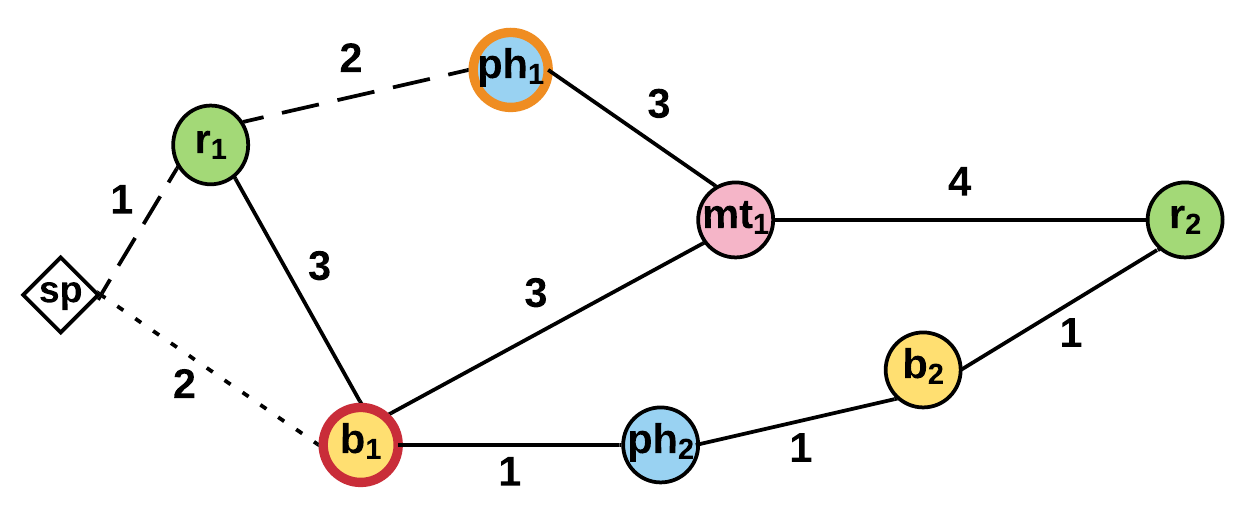
\includegraphics[scale=0.8]{Example_OR_1.png}
	\end{figure}
	
	\begin{table}[h]
		\centering
		\begin{tabular}{ |l|p{10cm}| } 
			\hline
			Step & Heap contents (PSR $R : length(r), r.notordered$) \\
			\hline
			\textcolor{red}{1} & \textcolor{red}{$(b_1 : 2, [ph])$} \\ 
			\hline
		\end{tabular}
	\end{table}

\end{frame}

\begin{frame}[noframenumbering]{Example: Step 1}
	$M = (b, r, ph)$, $ORDER = (1)$
	
	\begin{figure}[h]
		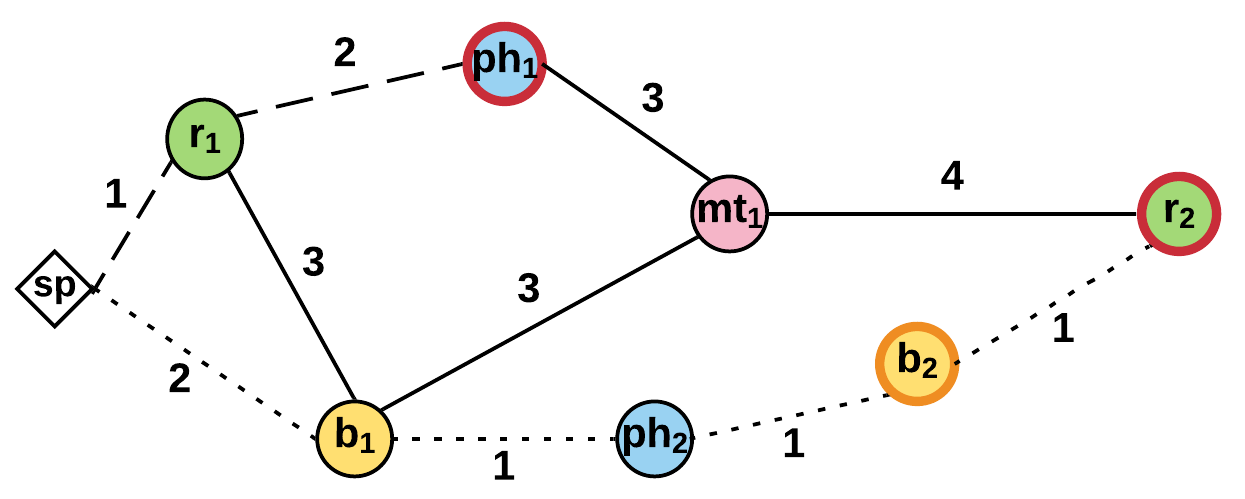
\includegraphics[scale=0.8]{Example_ORDER_2.png}
	\end{figure}
	
	\begin{table}[h]
		\centering
		\begin{tabular}{ |l|p{10cm}| } 
			\hline
			Step & Heap contents (PSR $R : length(r), r.notordered$) \\
			\hline
			1 & $(b_1 : 2, [ph])$ \\ 
			\hline
			\textcolor{red}{2} & \textcolor{red}{$(ph_1 : 3, [b])$}, \textcolor{red}{$(b_1, r_2 : 5, [ph])$} \\ 
			\hline
		\end{tabular}
	\end{table}

\end{frame}

\begin{frame}[noframenumbering]{Example: Step 6}
	$M = (b, r, ph)$, $ORDER = (1)$
	
	\begin{figure}[h]
		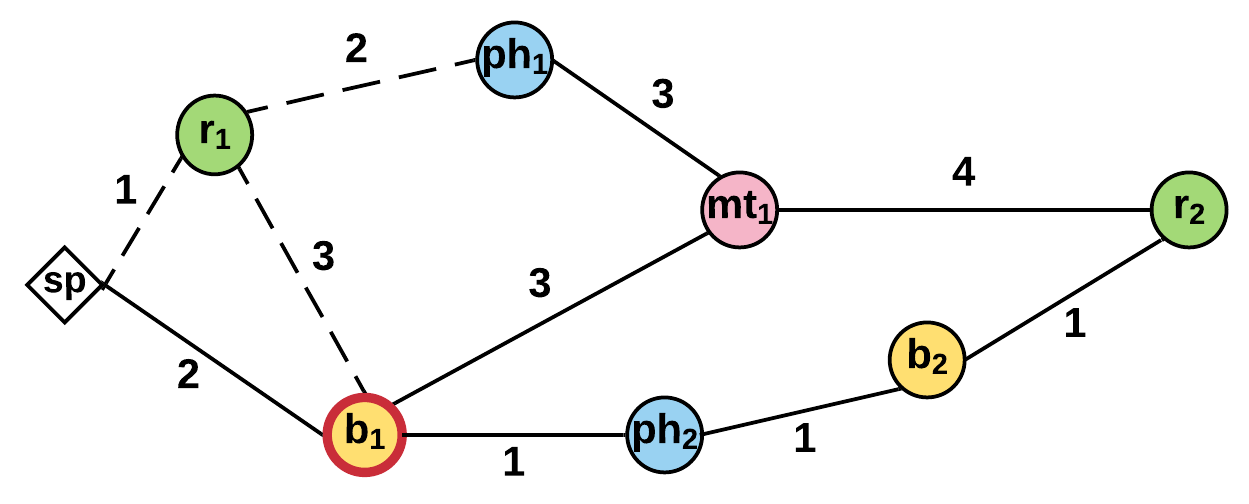
\includegraphics[scale=0.8]{Example_ORDER_6.png}
	\end{figure}
	
	\begin{table}[h]
		\centering
		\begin{tabular}{ |l|p{10cm}| } 
			\hline
			Step & Heap contents (PSR $R : length(r), r.notordered$) \\
			\hline
			5 & $(ph_1, r_1 : 5, [b]), (b_2, r_2 : 5, [ph]), (ph_2, r_2 : 5, [b]), (b_1, r_2 : 5, [ph])$ \\ 
			\hline
			\textcolor{red}{6} & $(b_2, r_2 : 5, [ph]), (ph_2, r_2 : 5, [b]), (b_1, r_2 : 5, [ph]),$ \textcolor{red}{$(ph_1, r_1, b_1 : 8, [])$} \\ 
			\hline
		\end{tabular}
	\end{table}

\end{frame}

\begin{frame}[noframenumbering]{Example: Step 12}
	$M = (b, r, ph)$, $ORDER = (1)$
	
	\begin{figure}[h]
		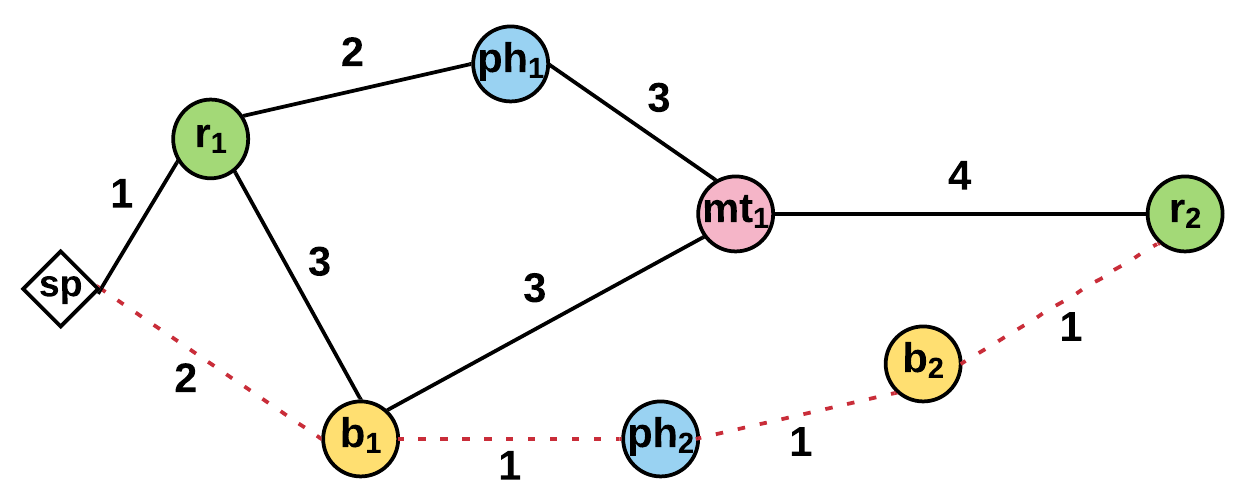
\includegraphics[scale=0.8]{Example_ORDER_12.png}
	\end{figure}
	
	\begin{table}[h]
		\centering
		\begin{tabular}{ |l|p{10cm}| } 
			\hline
			Step & Heap contents (PSR $R : length(r), r.notordered$) \\
			\hline
			10 & $(b_2, r_2 : 5, [ph]), (ph_2, r_2, b_2 : 6, []),$ \st{$(b_1, r_1, ph_1 : 7, [])$} $, (ph_2, r_1 :7, [b]), (b_2, r_1 : 9, [ph]), (ph_1, r_2 : 10, [b])$ \\ 
			\hline
			11 & $\textcolor{red}{(ph_2, r_2, b_2 : 6, [])}, (ph_2, r_1 :7, [b]), (b_2, r_1 : 9, [ph]), (ph_1, r_2 : 10, [b]),$ \st{$(b_2, r_2, ph_1 : 12, [])$} \\ 
			\hline
		\end{tabular}
	\end{table}

\end{frame}

%\begin{frame}{Example}
%	\begin{table}[]
%		\centering
%		\begin{tabular}{ |l|p{10cm}| } 
%			\hline
%			Step & Heap contents (PSR $R : length(r), r.notordered$) \\
%			\hline
%			1 & $(b_1 : 2, [ph])$ \\ 
%			\hline
%			2 & $(ph_1 : 3, [b]), (b_1, r_2 : 5, [ph])$ \\ 
%			\hline
%			3 & $(ph_2 : 3, [b]), (ph_1, r_1 : 5, [b]), (b_1, r_2 : 5, [ph])$ \\ 
%			\hline
%			4 & $(b_2 : 4, [ph]), (ph_2, r_2 : 5, [b]), (ph_1, r_1 : 5, [b]), (b_1, r_2 : 5, [ph])$ \\ 
%			\hline
%			5 & $(ph_1, r_1 : 5, [b]), (b_2, r_2 : 5, [ph]), (ph_2, r_2 : 5, [b]), (b_1, r_2 : 5, [ph])$ \\ 
%			\hline
%			6 & $(b_2, r_2 : 5, [ph]), (ph_2, r_2 : 5, [b]), (b_1, r_2 : 5, [ph]), (ph_1, r_1, b_1 : 8, [])$ \\ 
%			\hline
%			7 & $(b_1, r_2 : 5, [ph]), (b_2, r_2, ph : 5, [ph]), (ph_2, r_2 : 5, [b]), (b_2, r_2, ph_2 : 7, []),$ \st{$(ph_1, r_1, b_1 : 8, [])$} $, (b_2, r_1 : 9, [ph]), (ph_1, r_2 : 10, [b])$ \\ 
%			\hline
%			8 & $(b_2, r_2 : 5, [ph]), (ph_2, r_2 : 5, [b]), (b_1, r_1 : 5, [ph]), (b_2, r_2, ph_2 : 7, []), $ \st{$(b_1, r_2, ph_2 : 7, [])$} $, (b_2, r_1 : 9, [ph]), (ph_1, r_2 : 10, [b])$ \\ 
%			\hline
%			9 & $(b_1, r_1 : 5, [ph]), (b_2, r_2 : 5, [ph]), (ph_2, r_2, b_2 : 6, []),$ \st{$(b_2, r_2, ph_2 : 7, [])$} $, (ph_2, r_1 :7, [b]), (b_2, r_1 : 9, [ph]), (ph_1, r_2 : 10, [b])$ \\ 
%			\hline
%			10 & $(b_2, r_2 : 5, [ph]), (ph_2, r_2, b_2 : 6, []),$ \st{$(b_1, r_1, ph_1 : 7, [])$} $, (ph_2, r_1 :7, [b]), (b_2, r_1 : 9, [ph]), (ph_1, r_2 : 10, [b])$ \\ 
%			\hline
%			11 & $(ph_2, r_2, b_2 : 6, []), (ph_2, r_1 :7, [b]), (b_2, r_1 : 9, [ph]), (ph_1, r_2 : 10, [b]),$ \st{$(b_2, r_2, ph_1 : 12, [])$} \\ 
%			\hline
%		\end{tabular}
%	\end{table}
%\end{frame}